\documentclass[12pt, twoside]{article}
\input{../preamble}

\fancyhead[LE]{\thepage}
\fancyhead[RO]{Name: \hspace{4cm} \,\\ \hspace{2.9cm} \,}
\fancyhead[LO]{La Scuola d'Italia / Dr.\ Huson / IB Math: Probability \\* 5 March 2026}

\begin{document}
\subsubsection*{4.17 Quiz: Probability}
\begin{enumerate}[itemsep=0.1cm]


%--- Problem 1: Fully-labeled Venn diagram ---
\item In a group of 40 students, some play football ($F$) and some play basketball ($B$).
Six students play both sports. This information is shown in the following Venn diagram.

\begin{center}
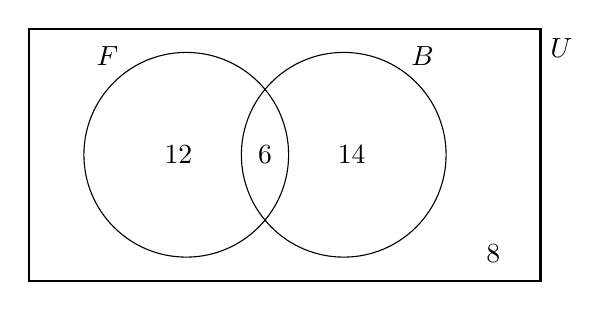
\begin{tikzpicture}
  \draw[thick] (0,0) rectangle (6.5,3.2);
  \node[anchor=north west] at (6.5,3.2) {$U$};
  \draw (2.0,1.6) circle (1.3cm);
  \node at (1.0,2.85) {$F$};
  \draw (4.0,1.6) circle (1.3cm);
  \node at (5.0,2.85) {$B$};
  \node at (1.9,1.6) {$12$};
  \node at (3.0,1.6) {$6$};
  \node at (4.1,1.6) {$14$};
  \node at (5.9,0.35) {$8$};
\end{tikzpicture}
\end{center}

\begin{enumerate}[itemsep=0.25cm]
  \item Write down the number of students in the group who play football. \hfill [2]
  \item One student from the group is chosen at random. Find the probability that
  \begin{enumerate}[label=(\roman*), itemsep=0.25cm]
    \item the student does not play football;
    \item the student plays football or basketball, but not both. \hfill [4]
  \end{enumerate}
\end{enumerate}

\begin{tikzpicture}
  \draw (0,0) rectangle (15.5,5);
  \foreach \y in {1,2,...,4} \draw[dotted] (0.5,\y)--(15,\y);
\end{tikzpicture}


%--- Problem 2: Mutually exclusive ---
\item Events $A$ and $B$ are mutually exclusive with
$\mathrm{P}(A) = 0.55$ and $\mathrm{P}(B) = 0.15$.

\begin{enumerate}[itemsep=0.25cm]
  \item Write down $\mathrm{P}(A \cap B)$. \hfill [1]
  \item Find $\mathrm{P}(A \cup B)$. \hfill [2]
\end{enumerate}

\begin{tikzpicture}
  \draw (0,0) rectangle (15.5,4);
  \foreach \y in {1,2,3} \draw[dotted] (0.5,\y)--(15,\y);
\end{tikzpicture}

\newpage

%--- Problem 3: Venn diagram ---
\item In a survey of 25 students, 18 own a bicycle and 7 own a scooter.
Three students own both, as shown in the following Venn diagram.
The values $\boldsymbol{p}$ and $\boldsymbol{q}$ represent numbers of students.

\begin{center}
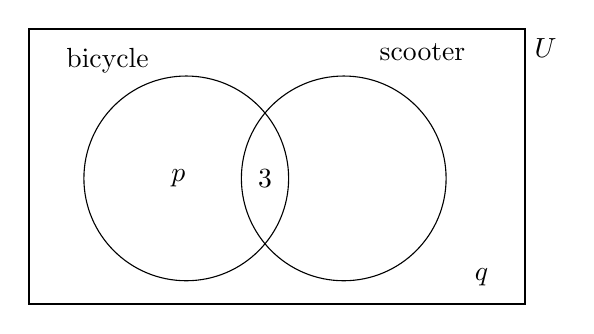
\begin{tikzpicture}
  \draw[thick] (0,0) rectangle (6.3,3.5);
  \node[anchor=north west] at (6.3,3.5) {$U$};
  \draw (2.0,1.6) circle (1.3cm);
  \node at (1,3.1) {bicycle};
  \draw (4.0,1.6) circle (1.3cm);
  \node at (5,3.2) {scooter};
  \node at (1.9,1.6) {$p$};
  \node at (3.0,1.6) {$3$};
  \node at (5.75,0.35) {$q$};
\end{tikzpicture}
\end{center}

\begin{enumerate}[itemsep=0.25cm]
  \item Find the value of $\boldsymbol{p}$. \hfill [1]
  \item Find the value of $\boldsymbol{q}$. \hfill [1]
  \item A student is chosen at random. Find the probability that the student
        owns a scooter but not a bicycle. \hfill [2]
\end{enumerate}
\vspace{0.2cm}

\begin{tikzpicture}
  \draw (0,0) rectangle (15.5,9);
  \foreach \y in {1,2,3,...,8} \draw[dotted] (0.5,\y)--(15,\y);
\end{tikzpicture}

\newpage
%--- Problem 4: Two-way table ---
\item The following table shows the sports and snack preferences of 20 students.

\renewcommand{\arraystretch}{1.8}
\begin{center}
\begin{tabular}{r|c|c|c}
    & Peanuts & Popcorn & Total \\
    \hline
    Mets fans    & 4  & 10 & 14 \\
    \hline
    Yankees fans & 2  & 4  & 6  \\
    \hline
    Total        & 6  & 14 & 20 \\
\end{tabular}
\end{center}

\begin{enumerate}[itemsep=0.25cm]
  \item Find the probability that a student chosen at random
        is a Yankees fan who likes popcorn. \hfill [2]
  \item Find the probability that a student is a Mets fan,
        given that they like peanuts. \hfill [2]
  \item Determine whether being a Mets fan and liking peanuts
        are independent events. Justify your answer. \hfill [2]
\end{enumerate}
\vspace{0.2cm}

\begin{tikzpicture}
  \draw (0,0) rectangle (15.5,9);
  \foreach \y in {1,2,3,...,8} \draw[dotted] (0.5,\y)--(15,\y);
\end{tikzpicture}


\newpage

%--- Problem 5: Tree diagram ---
\item A factory produces parts using two manufacturing processes.
Process $A$ produces $60\%$ of all parts and process $B$ produces the remaining $40\%$.
The probability that a part from process $A$ is defective is $0.05$.
The probability that a part from process $B$ is defective is $0.15$.

\begin{enumerate}[itemsep=0.4cm]
  \item Complete the tree diagram, showing all probabilities. \hfill [3]

  \begin{center}
  \begin{tikzpicture}
    % Branches — equal horizontal spans of 3.5 at both levels
    \draw (0,0) -- (3.5, 2.0);
    \draw (0,0) -- (3.5,-2.0);
    \draw (3.5, 2.0) -- (7.0, 3.5);
    \draw (3.5, 2.0) -- (7.0, 1.0);
    \draw (3.5,-2.0) -- (7.0,-1.0);
    \draw (3.5,-2.0) -- (7.0,-3.5);
    % First-level probability labels (above/below branch midpoints)
    \node[above] at (1.75, 1.0) {$0.6$};
    \node[below] at (1.75,-1.0) {$0.4$};
    % Junction labels — above-left/below-left to stay clear of outgoing branches
    \node[above left] at (3.5, 2.0) {\small Process $A$};
    \node[below left] at (3.5,-2.0) {\small Process $B$};
    % Second-level labels: above upward branches, below downward branches
    \node[above] at (5.25, 2.75) {$0.05$};
    \node[below] at (5.25, 1.50) {\rule{1.2cm}{0.4pt}};
    \node[above] at (5.25,-1.50) {\rule{1.2cm}{0.4pt}};
    \node[below] at (5.25,-2.75) {\rule{1.2cm}{0.4pt}};
    % Outcome labels
    \node[anchor=west] at (7.15, 3.5) {Defective};
    \node[anchor=west] at (7.15, 1.0) {Not defective};
    \node[anchor=west] at (7.15,-1.0) {Defective};
    \node[anchor=west] at (7.15,-3.5) {Not defective};
    % Combined probability blanks (students multiply along each path)
    \node[anchor=west] at (10.5, 3.5) {$=$ \rule{1.8cm}{0.4pt}};
    \node[anchor=west] at (10.5, 1.0) {$=$ \rule{1.8cm}{0.4pt}};
    \node[anchor=west] at (10.5,-1.0) {$=$ \rule{1.8cm}{0.4pt}};
    \node[anchor=west] at (10.5,-3.5) {$=$ \rule{1.8cm}{0.4pt}};
  \end{tikzpicture}
  \end{center}

  \item A part is selected at random. Find the probability that the part is
  \begin{enumerate}[label=(\roman*), itemsep=0.25cm]
    \item defective and from process $A$; \hfill [2]
    \item defective. \hfill [2]
  \end{enumerate}

  \item Given that a part is defective, find the probability that it came from
        process $A$. \hfill [3]
\end{enumerate}

\begin{tikzpicture}
  \draw (0,0) rectangle (15.5,5);
  \foreach \y in {1,2,...,4} \draw[dotted] (0.5,\y)--(15,\y);
\end{tikzpicture}

\newpage

%--- Problem 6: Two-step tree, no replacement ---
\item A drawer contains 8 black socks and 6 brown socks. Two socks are
taken from the drawer at random, one after the other, without replacement.

\begin{enumerate}[itemsep=0.25cm]
  \item Find the probability that both socks are black. \hfill [2]
  \item Find the probability that the two socks are the same colour. \hfill [4]
\end{enumerate}

\begin{tikzpicture}
  \draw (0,0) rectangle (15.5,11);
  \foreach \y in {1,2,...,10} \draw[dotted] (0.5,\y)--(15,\y);
\end{tikzpicture}

\end{enumerate}
\end{document}

Solutions
Problem 1 — Fully-labeled Venn diagram: 40 students, football (F) / basketball (B)
  - (a) Number who play football = 12 + 6 = 18
  - (b)(i)  P(not football) = (14 + 8)/40 = 22/40 = 0.55
  - (b)(ii) P(football or basketball, not both) = (12 + 14)/40 = 26/40 = 0.65

Problem 2 — Mutually exclusive: P(A) = 0.55, P(B) = 0.15
  - (a) P(A ∩ B) = 0  (definition of mutually exclusive)
  - (b) P(A ∪ B) = 0.55 + 0.15 = 0.70

Problem 3 — Venn diagram with p and q: 25 students, bicycle / scooter, 3 own both
  - (a) p = 18 - 3 = 15  (bicycle only)
  - (b) q = 25 - (18 + 7 - 3) = 3  (neither)
  - (c) P(scooter but not bicycle) = (7 - 3)/25 = 4/25 = 0.16

Problem 4 — Two-way table: 20 students, Mets/Yankees × peanuts/popcorn
  - (a) P(Yankees ∩ popcorn) = 4/20 = 0.2
  - (b) P(Mets | peanuts) = 4/6 = 2/3 ≈ 0.667
  - (c) P(Mets) × P(peanuts) = (14/20) × (6/20) = 0.7 × 0.3 = 0.21 ≠ 4/20 = 0.2
        → NOT independent

Problem 6 — Two-step, no replacement: 8 black socks, 6 brown (14 total)
  - (a) P(both black) = (8/14)(7/13) = 56/182 = 4/13 ≈ 0.308
  - (b) P(both brown) = (6/14)(5/13) = 30/182 = 15/91
        P(same colour) = 56/182 + 30/182 = 86/182 = 43/91 ≈ 0.473

Problem 5 — Tree diagram: factory parts, process A (60%) / process B (40%)
  - (a) Blank values: 0.95 (not defective | A),  0.15 (defective | B),  0.85 (not defective | B)
  - (b)(i)  P(defective ∩ A) = 0.6 × 0.05 = 0.030
  - (b)(ii) P(defective) = 0.030 + 0.4 × 0.15 = 0.030 + 0.060 = 0.090
  - (c) P(A | defective) = 0.030 / 0.090 = 1/3 ≈ 0.333
